Penelitian ini dilaksanakan sepenuhnya pada lingkungan simulasi berbasis Robot Operating System (ROS) dan Gazebo. Pendekatan simulasi dipilih untuk menjamin reproduktivitas eksperimen, memudahkan pengendalian variabel pengujian, serta memungkinkan pelaksanaan pengujian berulang pada kondisi yang identik (\cite{Adiuku2024}). Lingkungan simulasi yang digunakan dirancang untuk merepresentasikan skenario navigasi robot bergerak otonom pada area dalam ruangan dengan berbagai konfigurasi obstacle statis maupun dinamis. Subbab ini menjelaskan perangkat keras, perangkat lunak, serta lingkungan simulasi yang digunakan selama penelitian.

\subsection{Perangkat Keras}
\label{sec:perangkat_keras}

Meskipun penelitian ini tidak melibatkan robot fisik secara langsung, proses simulasi tetap memerlukan sumber daya komputasi yang memadai untuk menjalankan simulator, sistem navigasi, dan pemrosesan data sensor secara \textit{real-time}. Selain itu, model sensor yang digunakan dalam simulasi dirancang untuk merepresentasikan karakteristik sensor yang umum digunakan pada robot bergerak otonom.

\subsubsection*{a. Komputer Host}

Seluruh simulasi dan pengolahan data dilakukan pada komputer host dengan spesifikasi yang disajikan pada Tabel~\ref{tab:spesifikasi_komputer_host}. Spesifikasi tersebut dinilai memadai untuk menjalankan simulasi Gazebo, pemrosesan data sensor, serta pencatatan data eksperimen secara bersamaan selama proses pengujian berlangsung.

\begin{table}[H]
\centering
\caption{Spesifikasi komputer host yang digunakan dalam penelitian}
\label{tab:spesifikasi_komputer_host}
\begin{tabular}{ll}
\toprule
\textbf{Komponen} & \textbf{Spesifikasi} \\
\midrule
Sistem Operasi & Ubuntu 20.04 LTS (64-bit) \\
Prosesor & AMD Ryzen 5 6600H \\
RAM & 16 GB \\
GPU & NVIDIA GeForce RTX 3050 Laptop GPU (4 GB VRAM) \\
\bottomrule
\end{tabular}
\end{table}

\subsubsection*{b. Model Robot}

Robot yang digunakan dalam penelitian ini adalah \texttt{CAD\_ASR\_WITH\_OMNI}, yaitu robot be\-roda tiga dengan konfigurasi omnidirectional (holonomik) yang memungkinkan robot bergerak ke berbagai arah tanpa harus mengubah orientasi badan robot terlebih dahulu. Model robot didefinisikan menggunakan \textit{Unified Robot Description Format} (URDF) dan dijalankan pada lingkungan simulasi Gazebo melalui antarmuka ROS (\cite{Adiuku2024}).

Untuk keperluan navigasi, robot direpresentasikan menggunakan \textit{footprint} berbentuk per\-segi dengan dimensi 0,54 m $\times$ 0,64 m. Representasi \textit{footprint} tersebut digunakan oleh sistem \textit{costmap} untuk menentukan ruang bebas, memperhitungkan jarak aman terhadap obstacle, serta mendukung proses perencanaan lintasan selama navigasi berlangsung.

\subsubsection*{c. Sensor LiDAR}

Sensor utama yang digunakan dalam penelitian ini adalah LiDAR dua dimensi yang menghasilkan data pindaian lingkungan dalam format \texttt{sensor\_msgs/LaserScan}. Sensor ini memiliki cakupan sudut horizontal sebesar 360$^\circ$ dengan frekuensi pembaruan 40 Hz dan digunakan sebagai sumber utama informasi geometris lingkungan.

Data LiDAR dimanfaatkan untuk mendeteksi obstacle, menghitung jarak terhadap obstacle terdekat, serta mendukung proses perencanaan lintasan robot. Namun demikian, LiDAR dua dimensi hanya melakukan pemindaian pada satu bidang horizontal sehingga memiliki keterbatasan dalam mendeteksi obstacle yang seluruh profilnya berada di luar bidang pindai sensor. Keterbatasan tersebut menyebabkan munculnya area \textit{blind-spot} yang menjadi salah satu permasalahan utama pada penelitian ini (\cite{Fagundes2024,Kibii2022}).

\subsubsection*{d. Kamera Termal}

Selain LiDAR, penelitian ini menggunakan kamera termal sebagai sensor pelengkap untuk meningkatkan kemampuan persepsi lingkungan. Kamera termal menghasilkan citra berbasis distribusi intensitas panas yang direpresentasikan dalam format \textit{grayscale}. Berbeda dengan LiDAR yang mengandalkan informasi geometris, kamera termal mampu mengidentifikasi objek berdasarkan karakteristik termalnya sehingga tetap dapat mendeteksi obstacle tertentu yang tidak teramati oleh LiDAR (\cite{Choi2023}).

Informasi yang diperoleh dari kamera termal digunakan untuk mengestimasi kondisi area di depan robot serta mendukung proses pembentukan informasi traversability lingkungan. Pendekatan integrasi LiDAR dan kamera termal banyak digunakan pada sistem robotika modern karena kedua sensor memiliki karakteristik pengamatan yang saling melengkapi (\cite{Schichler2025}).

Spesifikasi sensor yang digunakan dalam simulasi ditunjukkan pada Tabel~\ref{tab:spesifikasi_sensor}.

\begin{table}[H]
\centering
\caption{Spesifikasi sensor yang digunakan dalam simulasi}
\label{tab:spesifikasi_sensor}
\begin{tabular}{llll}
\toprule
\textbf{Parameter} & \textbf{LiDAR} & \textbf{Kamera Termal} & \textbf{Satuan} \\
\midrule
Frame pemasangan & laser & thermal\_link & -- \\
Posisi dari base\_link (x, y) & (0,147; 0,362) & (0,170; 0,660) & m \\
Orientasi yaw & 0 & -0,52 & rad \\
Cakupan sudut horizontal & 360$^\circ$ & 90$^\circ$ & -- \\
Resolusi data & 720 sampel & 640 $\times$ 480 & -- \\
Jangkauan minimum & 0,05 & 0,10 & m \\
Jangkauan maksimum & 12,0 & 100,0 & m \\
Frekuensi pembaruan & 40 & 10 & Hz \\
Keluaran data & LaserScan & Citra termal grayscale & -- \\
\bottomrule
\end{tabular}
\end{table}

\subsection{Perangkat Lunak}
\label{sec:perangkat_lunak}

Pengembangan sistem dilakukan menggunakan beberapa perangkat lunak yang saling terintegrasi dalam ekosistem ROS. Daftar perangkat lunak dan modul utama yang digunakan dalam penelitian ini disajikan pada Tabel~\ref{tab:perangkat_lunak}.

\begin{table}[H]
\centering
\caption{Perangkat lunak dan modul utama yang digunakan}
\label{tab:perangkat_lunak}
\begin{tabular}{p{3.5cm}p{2cm}p{7cm}}
\toprule
\textbf{Komponen} & \textbf{Versi} & \textbf{Fungsi} \\
\midrule
Ubuntu & 20.04 LTS & Sistem operasi host \\
ROS Noetic & Noetic & Middleware komunikasi sistem \\
Gazebo & 11 & Simulator robot dan lingkungan \\
NavfnROS & 1.17.3 & Perencanaan lintasan global \\
APFPlanner & Kustom & Perencanaan lintasan lokal \\
OpenCV & 4.2.0 & Pemrosesan citra termal \\
semantic\-\_thermal.py & Kustom & Segmentasi citra termal \\
thermal\_feature\-\_extractor.py & Kustom & Ekstraksi fitur traversability \\
thermal\_blindspot\-\_to\_scan.py & Kustom & Pembentukan \textit{virtual scan} termal \\
experiment\-\_logger.py & Kustom & Pencatatan data eksperimen \\
\bottomrule
\end{tabular}
\end{table}

ROS Noetic digunakan sebagai \textit{middleware} yang menghubungkan seluruh komponen sistem melalui mekanisme komunikasi berbasis topik. Sementara itu, Gazebo berperan sebagai simulator yang menyediakan lingkungan virtual, model robot, serta emulasi sensor yang digunakan selama proses pengujian. Integrasi ROS dan Gazebo banyak digunakan dalam penelitian robotika karena mendukung pengembangan sistem secara modular dan reproduktif (\cite{Macenski2022,Adiuku2024}).

Selain perangkat lunak utama, penelitian ini juga memanfaatkan beberapa pustaka pendukung seperti NumPy untuk komputasi numerik, OpenCV untuk pemrosesan citra, Pandas untuk pengelolaan data eksperimen, serta SciPy untuk analisis statistik hasil pengujian.

\subsection{Lingkungan Simulasi}
\label{sec:lingkungan_simulasi}

\subsubsection*{a. Model Robot \texttt{CAD\_ASR\_WITH\_OMNI}}

Lingkungan simulasi menggunakan model robot \texttt{CAD\_ASR\_WITH\_OMNI} yang telah dileng\-kapi dengan sensor LiDAR dan kamera termal. Kedua sensor ditempatkan pada bagian depan robot untuk memaksimalkan area pengamatan ke arah pergerakan robot. Visualisasi model robot dan posisi pemasangan sensor ditunjukkan pada Gambar~\ref{fig:model_robot_sensor}.

\begin{figure}[H]
\centering
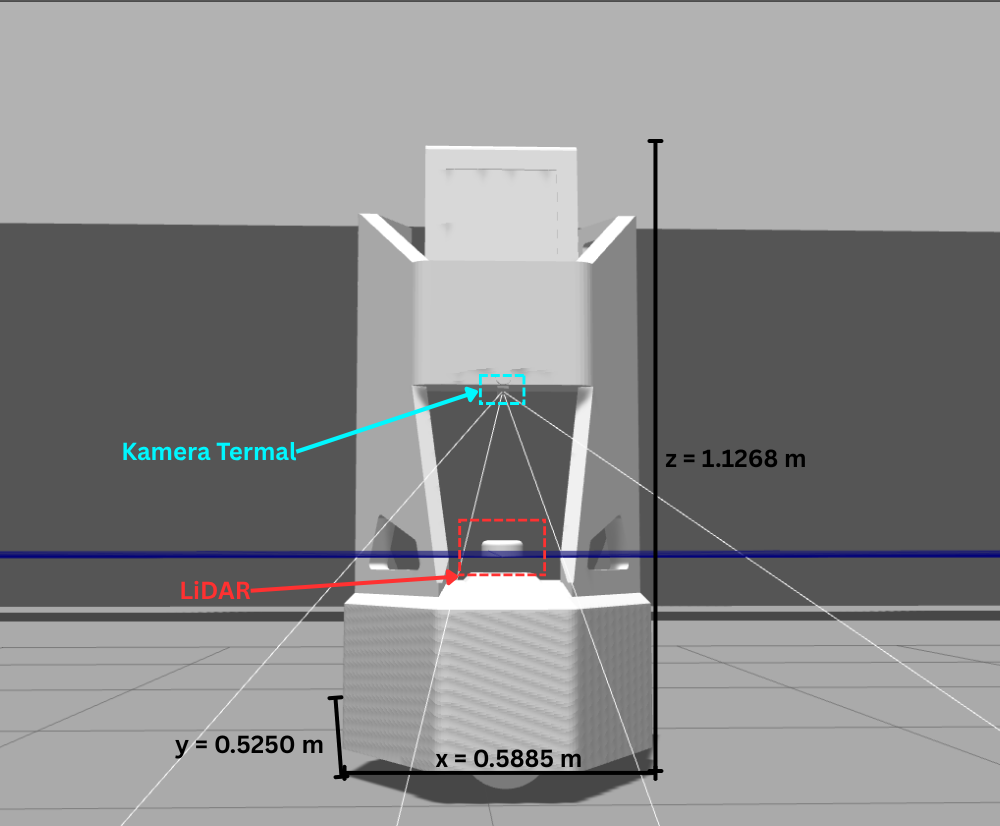
\includegraphics[width=0.5\textwidth]{gambar/3.2_robot_model.png}
\caption{Model robot \texttt{CAD\_ASR\_WITH\_OMNI} dan penempatan sensor.}
\label{fig:model_robot_sensor}
\end{figure}

\subsubsection*{b. Peta Lingkungan Simulasi}

Navigasi robot dilakukan pada lingkungan dalam ruangan yang direpresentasikan menggunakan \textit{occupancy grid map}. Peta disediakan melalui paket \textit{map\_server} dan digunakan oleh \textit{global planner} untuk menghasilkan lintasan menuju tujuan.

Peta yang digunakan pada penelitian ini adalah \texttt{grit\_1\_edited\_2}, yang memuat informasi area bebas, area terhalang, dan batas lingkungan simulasi. Representasi peta tersebut menjadi dasar pembentukan \textit{global costmap} yang digunakan oleh sistem navigasi.

\subsubsection*{c. Lokalisasi Robot}

Lokalisasi robot dilakukan menggunakan komponen \textit{fake\_localization}, yaitu metode loka\-lisasi yang memanfaatkan posisi \textit{ground-truth} dari simulator Gazebo sebagai estimasi pose robot pada peta. Pendekatan ini dipilih karena penelitian berfokus pada evaluasi sistem navigasi dan penghindaran obstacle, bukan pada akurasi estimasi posisi robot.

Dengan menggunakan \textit{fake\_localization}, pengaruh kesalahan lokalisasi dapat dieliminasi sehingga perbedaan performa yang diamati antara konfigurasi pengujian berasal dari meka\-nisme navigasi yang digunakan, bukan dari ketidakpastian estimasi posisi robot.

\subsubsection*{d. Obstacle Pengujian}

Penelitian ini menggunakan beberapa jenis obstacle yang ditempatkan pada lingkungan simulasi untuk merepresentasikan kondisi navigasi yang berbeda. Karakteristik obstacle yang digunakan disajikan pada Tabel~\ref{tab:spesifikasi_obstacle}.

\begin{table}[H]
\centering
\caption{Spesifikasi obstacle yang digunakan dalam simulasi}
\label{tab:spesifikasi_obstacle}
\begin{tabular}{llll}
\toprule
\textbf{Nama Model} & \textbf{Jenis} & \textbf{Radius} & \textbf{Terdeteksi LiDAR} \\
\midrule
obstacle\_cat & Statis & 0,18 m & Tidak \\
obstacle\_human\_1 & Statis/Dinamis & 0,25 m & Ya \\
obstacle\_human\_2 & Statis/Dinamis & 0,25 m & Ya \\
obstacle & Statis & 0,25 m & Ya \\
\bottomrule
\end{tabular}
\end{table}

Obstacle \texttt{obstacle\_cat} digunakan untuk merepresentasikan obstacle berprofil rendah yang berada pada area \textit{blind-spot} LiDAR. Sebaliknya, obstacle manusia dan obstacle umum memiliki dimensi yang cukup tinggi sehingga dapat dideteksi secara langsung oleh sensor LiDAR. Pada skenario dinamis, obstacle manusia digerakkan secara periodik untuk mensimulasikan keberadaan objek bergerak pada lingkungan navigasi robot.